
\documentclass[11pt,a4paper]{article}
\usepackage[hyperref]{naaclhlt2019}
\usepackage{times}
\usepackage{latexsym}
\usepackage{graphicx}

\usepackage{url}

\aclfinalcopy 

\title{Deep NLP for Author Profiling: Bot and Gender Detection}

\author{Christopher Watson \\
  {\tt chrwatson@cs.umass.edu} \\\And
  Emre Eryigit \\
  {\tt eeryigit@umass.edu} \\\And
  Forsad Al Hossain\\
  {\tt email@domain} \\}
  
% \setlength\textwidth{16.0cm}
\date{3/1/2019}

\begin{document}
\maketitle

\section{Introduction}
Tell us what problem you're going to work on. Provide some motivation for your idea: why is it interesting? Does it have any practical significance? 

Some general guidelines for this proposal document: 2 pages minimum for translation, 3 pages For ``choose your own projects'', due Mar 1. Please use this LaTeX template to write your proposal.

\section{Related work}

\noindent\textit{For both projects:} 
Check out papers at ACL/EMNLP/NAACL/TACL. Make sure to properly cite them. You can cite a paper parenthetically like this~\cite{andrew2007scalable} or use the citation as a proper noun, as in ``\newcite{borsch2011} show that...'' If you're not familiar with LaTeX, you'll have to add entries to \emph{yourbib.bib} to get them to show up when you cite them. 

\noindent\textit{For MT:} pick two papers on neural MT from ACL/EMNLP/NAACL/TACL and describe what they do. You may also choose papers from non-neural MT that you'd like to  extend to the neural setting.

\noindent\textit{For ``choose your own project'':}
Have others worked on this idea or related ideas? Clearly describe the some of these approaches, along with their pros and cons. You need to have at least five citations to related papers here. 

\section{Your approach}
How do you plan to solve the problem you chose? How will you approach it differently from previous work?

\noindent\textit{For ``choose your own project'':} remember that this project should take $\sim 2$ months of work! 

\paragraph{What baseline algorithms will you use?}
Our baseline algorithms will be a bag of words, deep averaging network. We will compare this to more complex models like LSTM with attention.

\subsection{Milestones \& Schedule}
 Project Schedule:
\begin{enumerate}
    \item Acquire and preprocess data (1 week)
    \item Generate word embeddings(1 week)
    \item Train LSTM w/ attention model(1 weeks)
    \item Write progress report! (1 week) (due Apr 1)
    \item Analyze the output of the model, do an error analysis (2 weeks)
    \item Work on final report and presentation (2 weeks)
\end{enumerate}


\section{Data}
We are using the PAN @ CLEF 2019 data set for Bots and Gender profiling. The corpus contains a total of 412,000 tweets. The data contains 4120 unique twitter users. Each user has a separate XML file containing 100 tweets.
The organizers have extracted the textual data from the tweets, but have not done any other pre-processing. All text is in raw form. This means some data cleaning will need to be performed before it is fed to the model. 
The ground truth data is given in a separate file, truth.txt. the format can be seen in Figure 2. Each line contains the AuthorID, human/bot, and male/female/bot fields.



\begin{figure}[t]
    \centering
    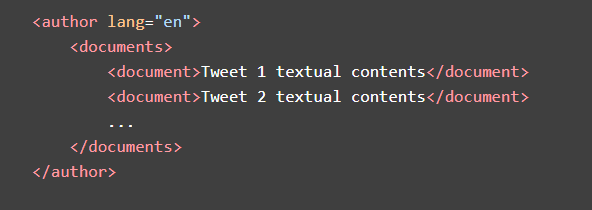
\includegraphics[width=0.5\textwidth]{figs/xml.png}
    \caption{XML file format.}
    \label{fig:data_example}
\end{figure}

\begin{figure}[t]
    \centering
    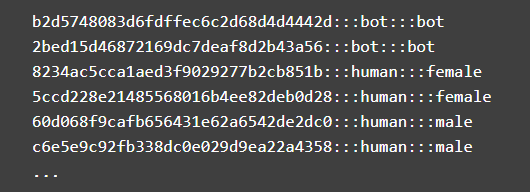
\includegraphics[width=0.5\textwidth]{figs/truth.PNG}
    \caption{Format of ground truth file, truth.txt.}
    \label{fig:data_example}
\end{figure}


\section{Tools}

The tweets from the PAN dataset are in raw form. This means that we will need to clean the data. Common data cleaning in previous years has included the removal or normalization of Twitter-specific elements such as URLs, user mentions, and hashtags. We may also lowercase the text, expand contractions, and remove punctuation, character flooding, and stopwords.

We will parse the words and using word2vec for our pre-trained word embeddings. 

Our deep learning model will be built using the Keras framework with a Tensorflow backend. We will train our models on free resources provided by Google Colab. 


\bibliographystyle{apalike}
\footnotesize
\bibliography{yourbib}


\end{document}
